\cleardoublepage
\setlist[enumerate,1]{%
  label=\arabic*.,
}

\newlist{inlinelist}{enumerate*}{1}
\setlist*[inlinelist,1]{%
  label=(\roman*),
}



\chapter{State of the Art}\label{sec:sota}\minitoc\vspace{.5cm}
\index{SotA}

\section{Introduction}
This chapter provides an understanding of the relevant terms, technologies, and standards in the field of Internet of things and Semantic interoperability. It starts with an introduction to the Internet of things with specifying its visions and the standardization efforts in this research area. Afterward, the most relevant standardization work of the IoT is presented. Eventually, after introducing the semantic web and semantic technology, the Semantic Web stack for the IoT is discussed, and the appropriate ontologies created for IoT are given. Finally, the openMTC platform is introduced as well as its architecture and most relevant features.

\section{Internet of Things}\index{Related Area}

In 1998, Kevin Ashton introduced the paradigm "Internet of things" (IoT)~\cite{bookiot}. Since then, this novel paradigm has attracted massive attention in academia as well as in industry~\cite{hindi}. \par
The IoT is intended to add a new dimension to the world of information and communication by defining a network in which physical devices have their virtual representation on the Internet, thus enabling the exchange of data between physical things, applications, and people. This interconnection allows the intercommunication and handling of things by other things or by humans, leading to the automation of different tasks and scenarios~\cite{gazi}. A thing can refer to wide variety of physical objects, from a humidity sensor at a farm to a heart rate monitoring device or a motor in a space station. It can refer virtually to a mobile phone application or enterprise resource planning software running in the cloud. This new dimension in the communications world is illustrated in the following: figure~\ref{fig:contrib2:d}

\begin{figure}[htbp]
    \centering
    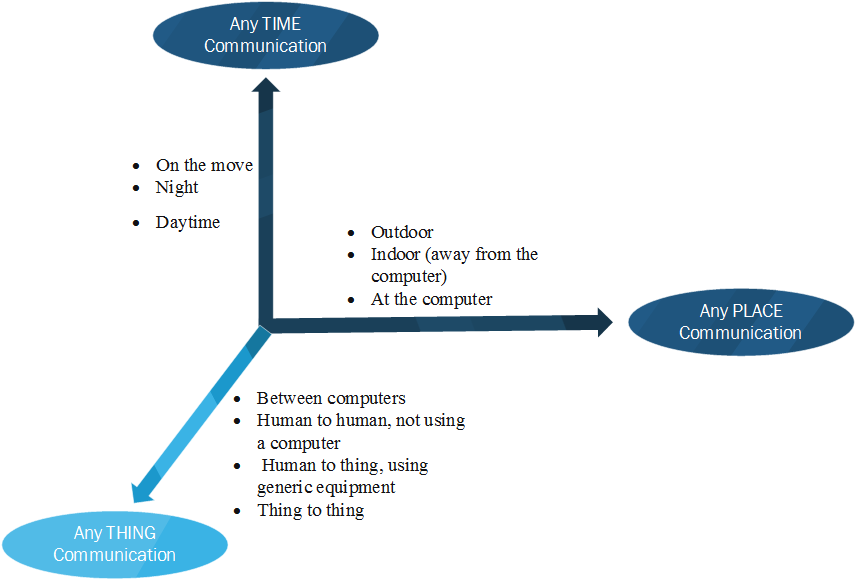
\includegraphics[width=1\textwidth]{resources/images/dimonsion}
    \caption{The new dimension introduced in the Internet of things adapted from~\cite{gazi} }\label{fig:contrib2:d}
\end{figure}
In this context, the IoT will have, in the near future, a massive impact on the lives and behavior of its users. By enabling smart homes, smart offices, e-health, and smart learning, the IoT will affect not only the private lives of everyday users but also their working environments. Similarly, from the point of view of business, the IoT will have a visible impact on industrial manufacturing, automation, logistics, business management, and intelligent transportation systems for people and goods.

\subsection{Concepts of IoT}

There are several IoT definition presented by the research communities which they derived it from the syntactical composition of the term. The first term, as shown previously, consist of "Internet" and the second term of "Things." Each term provides a particular signification. For instance, the term "Internet" shifts toward a network-oriented vision of IoT while the term "Things" concentrates on integrating general objects into a common framework [2]. Putting those two terms together proposes by its meaning a new level of innovation into the Information and communications technology (ICT) world. From this point of view, the IoT semantically means a network of connected uniquely addressable object based on standards communication protocols~\cite{semanticiot}. This means that there is a tremendous number of complex interconnected objects involved in the process. As introduced in the previous chapter, unique identification of all this heterogeneous resources or objects and the representation and storing of the exchanged information and data is one of the main challenges facing the IoT. For this reasons, the third perspective of the IoT was defined as the semantic integration. All three of those three visions of IoT are presented in Figure~\ref{fig:contrib2:vision}.
\begin{figure}[htbp]
    \centering
    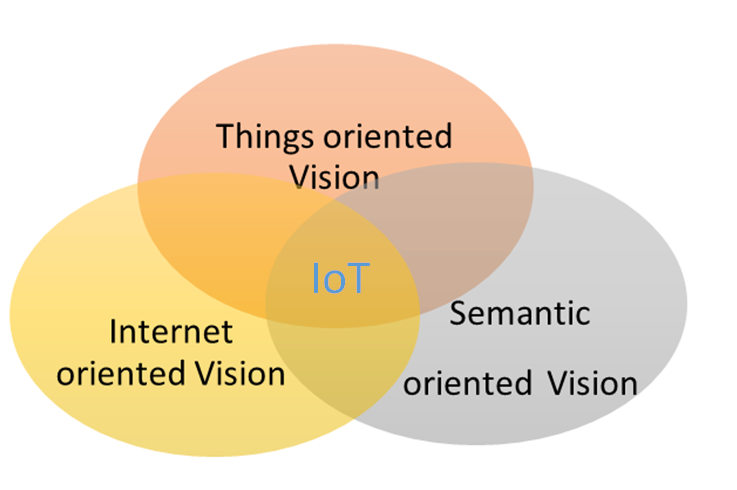
\includegraphics[width=1\textwidth]{resources/images/vision}
    \caption{Convergence of various visions of IoT adapted from~\cite{semanticiot} }\label{fig:contrib2:vision}
\end{figure}

From the perspective of "Things," the focus of IoT is on how to uniquely identify every object using specifications of the Electronic Product Code (EPC). Those objects are any things traceable using sensors and RFID technologies. Therefore, this vision depends mainly on sensor-based networks and RFID-based sensor networks~\cite{vision2}.\par
While the perspective of "things" aims at integrating various objects into a common framework, the perspective of "Internet" focuses on making smart objects interconnected. Since IP is a lightweight protocol that already connects a large number of communicating devices, it is used as well to connect heterogeneous objects~\cite{vision2}. In this context, the sensor-based object can be identified by an understandable format. This format is then uniquely identified, and its attributes are monitored as needed. \par
As mentioned earlier in this section and the previous chapter, semantics are also proposed as an IoT vision. This vision aims at providing interoperability between things in the IoT. Here is needed a general vision of processing the raw data into meaningful data and of a sealed detachment of data and their interpretation.

\subsection{Generic Architecture of IoT}

The implementation of the IoT is based on an architecture which consists of various layers. The application and business layers are presented at the top of this architecture while the field of perception layer is presented at the bottom. In this context, each component of the modern society--such as industries, enterprise, societies, institutes, and governments--is able to design the layered architecture of the IoT according to their requirements. Generally, the generic layered architecture for IoT is divided into five layers as shown in Figure~\ref{fig:contrib2:layer}. The layered architecture presented herein is proposed in~\cite{res1} and ~\cite{res2}.
\begin{figure}[htbp]
    \centering
    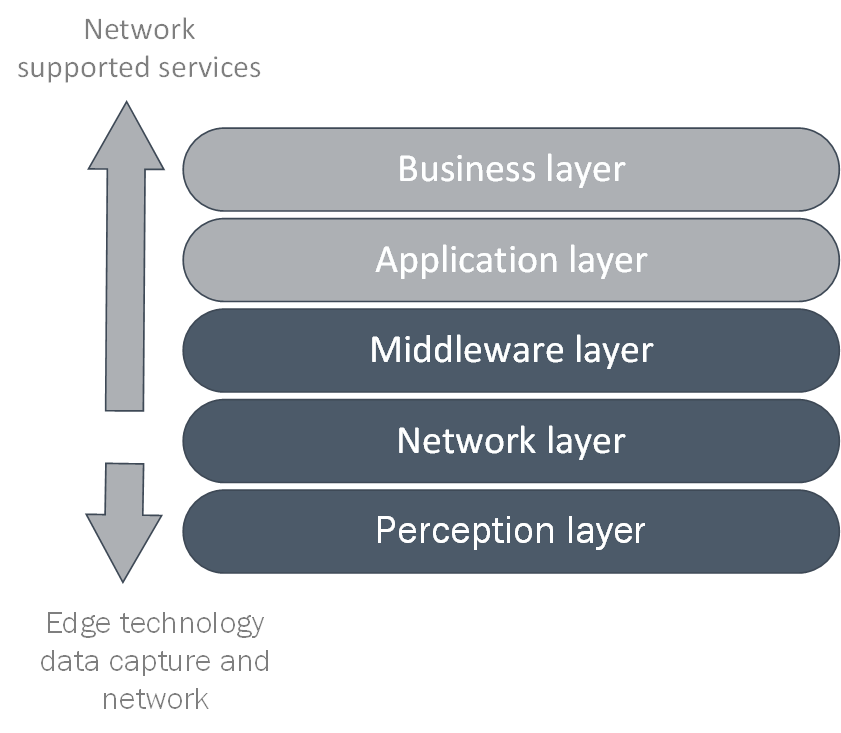
\includegraphics[width=.9\textwidth]{resources/images/iotarchi}
    \caption{The IoT Architecture inspired from~\cite{hindi} and~\cite{rep2}}\label{fig:contrib2:layer}
\end{figure}

The functionalities of the different layers are presented briefly in the following:
\begin{itemize}
\item \textbf{Business Layer:} Since that the real IoT technology success depends mainly on the business model in use, this layer is responsible for building business models, flow charts, and graphs based on the various data received from the Application layer. From this perspective, this layer has a significant role in determining the business strategies and future actions~\cite{archi}.
Application Layer: This layer represents all the different set of Application implemented by the IoT such as e-health, smart home, intelligent transportation system, etc. In a nutshell, this layer is responsible for managing applications based on the information retrieved from the set of objects processed in the Middleware layer.
\item \textbf{Middleware Layer:} This layer is responsible for managing the various services of the devices connected to the IoT system where each device is implementing a different type of service. It also stores the information and data received from the Network layer.\par
\item \textbf{Network Layer:} This layer is responsible for transferring the information and data provided by different devices and sensors from the Perception layer to the Middleware layer. In this context, the transmission medium can be wireless or wired. It also can be through various connectivity technologies such as Wifi, Bluetooth, ZigBee, etc.  
\item \textbf{Perception Layer:} This layer is responsible for the identification and collection of accurate information of sensor devices. This information varies depending on the sensors type. It can provide location, temperature, humidity, motion, etc. Afterward, this layer transfer that information to the Network layer.
\end{itemize}
\subsection{Standardization}
As presented previously, in IoT there are various technologies and components involved in data processing that have a particular data format and use different protocols. These factors make the exchange of data and communication among interconnected elements, with the intention of a combined processing of the information, a very complex task~\cite{booksd}. Therefore it is necessary that data representation, protocols, and interfaces are standardized. \par 
From this point of view, standards in IoT should be designed to meet the requirements of a various range of industries, societies, and even individual users. The design process should focus on enabling a bidirectional communication and information exchange between things. It should also emphasize their environment more and their representation in the virtual cloud from where diverse IoT applications are able to monitor, control, and assist them. As a result, standards in IoT should be created not only to support a broad range of applications but also to consider the network capacity as well as the energy efficiency~\cite{hindi}.  It is also necessary to take various regulations into consideration while designing a standard for IoT and to ensure sufficient capacity for expansion. \par
In this regard, designing a standard specified for IoT faces the interoperability issue as well. Therefore, IoT standard should ensure global interoperability between things that make use of radio spectrum in IoT. \par
In this context of IoT paradigm, at large, it is evident that the standardization of IoT is a fundamental part of the future Internet definition. This statement was already made by the cluster of European research and development projects on IoT (CERP-IoT)~\cite{fromhindi}.\par
From this perspective, there are various exciting standardization efforts being carried out by different governments and the private sector. The most relevant standardization efforts of the IoT that provide means in its design to solve the interoperability challenge are considered in the next section.

%Standards should be designed to support a wide range of applications and address common requirements from a wide range of industry sectors as well as the needs of the environment, society and individual citizens. Through consensus processes involving multiple stakeholders, it will be possible to develop standardized semantic data models and ontologies, common interfaces and protocols, initially defined at an abstract level, then with example bindings to specific cross-platform, cross-language technologies such as XML, ASN.1, web services etc. The use of semantic ontologies and machine-readable codification should help to overcome ambiguities resulting from human error or differences and misinterpretation due to different human languages in different regions of the world, as well as assisting with cross-referencing to additional information available through other systems.
\section{Standards For The Internet of Things }\index{Related Area 2}
Based on the understanding of the vision, architecture and the standardization mechanism of IoT provided in the previous section, this section focus on the organizations works on standardization process of IoT. Accordingly, this section covers only the standards that provide a definition for IoT and work on IoT as well.

\subsection{OPC Unified Architecture}

Based on the knowledge gained from the previous section, in order to realize the vision of IoT, it is required to create a global communication standard for the central components. Furthermore, it is required as well as to provide a means to manage bi-directional communication by enabling a publish/subscribe model for the low resource and a secure connection adapted for the client/server communication model~\cite{bookua}. This bi-directional communication is intended to send various commands to actors. Moreover, information is supposed to be accompanied by semantic information that represents the data and its purpose, which guarantee the best usage of the data. From this perspective, the Open Platform Communications (OPC) created a standard called Unified Architecture (OPC UA), which offers a solution for those requirements on the vertical layers for remote device access.

OPC Foundation provides various standards for data exchange, such as OPC DA specification for accessing current data, OPC HDA for accessing historical data, and OPC A&E for accessing alarms and events. The latest standard created by the OPC is the OPC UA. This standard was originally formed to enhance the Classic OPC with data modeling capabilities by providing a common, object-oriented paradigm for all OPC data~\cite{bookua}. As specified by this standard, the transport of data is mainly done by using web services based on various standards such as SOAP and HTTP or by using an optimized binary TCP protocol~\cite{bookua}. \par

OPC UA builds on the data transportation and information modeling. Thus, it aims at providing interoperability and platform-independency in the communication between applications by providing different possibilities to expose the semantics of the data provided by the Classic OPC~\cite{bookua}. One type of data provided by the OPC is the pressure measurement measured by a pressure sensor. Using the OPC UA standard, it is possible to present information in addition to the data provided by the Classic OPC. Thus, it is feasible to provide information about the type of sensor device that provided the measured temperature. This information is exposed within the OPC AU standard in a hierarchy specified for device types. Hence, OPC UA clients are capable of retrieving the information of the devices they are dealing with~\cite{bookua}. From this perspective, OPC UA provides means for different clients to process highly advanced tasks by interpreting the semantics of the provided data. \par
The OPC UA specifications provide the infrastructure to the information model. Those specifications are created to facilitate the lives of OPC UA clients by providing specifications usable by different vendor-specific OPC UA servers~\cite{bookua}. Currently, the OPC Foundation is working on defining the base model that presents the device information.\par
\subsubsection{Information Modeling}
 Based on the understanding of the previous section, the OPC UA standard is about information and data modeling. From this point of view, within this section the base principles of information modeling in OPC UA are highlighted in the following:
\begin{itemize}
\item \textbf{The use of object-oriented techniques:} those techniques which include type hierarchies and inheritance allows clients to handle all the various instance of the same type in the same way. Moreover, using the type hierarchies provide means to the user to work with the types needed and ignore the more specialized information.
\item \textbf{Accessing the type information the same way as instances:} by exposing the type information provided by the OPC UA server it is possible within the OPC UA standardization to access them in the same way as accessing instances. 
\item \textbf{Connect information in different ways:} OPC UA allows the connection among various information using a broad-meshed network of nodes. The OPC UA standard enables the use of different hierarchies exposing different semantics and references between nodes of those hierarchies. From this perspective, depending on the use case, it is possible to organize the information as needed. 
\item \textbf{Extensibility:} When it comes to information modeling, it is possible to extend the functionality of OPC UA by using various methods. In this context, it is possible for example to specify additional types of references defining relations between nodes and the definition of new methods that extends the functionality of OPC UA.
\item \textbf{Unlimited possibilities to model information:} Instead of mapping the model information to a different model, the OPC UA provide an unlimited methods to uniquely model information.
\item \textbf{Information modeling in server side only:} The information modeling is always performed on an OPC UA servers, and not on client-side. In the other hand, it is possible to manipulate them from more than one OPC UA clients.
\end{itemize}
\subsubsection{OPC UA Architecture }
he OPC UA architecture is based mainly on the communication stack between a server and the client(s). The purpose of this communication stack is to ensure encoding and decoding message requests and responses between the server and the client. Additionally, various communication stacks are able to work together only if they have the same technology mapping. This architecture is illustrated in Figure~\ref{fig:contrib2:ua}.\par
\begin{figure}[htbp]
    \centering
    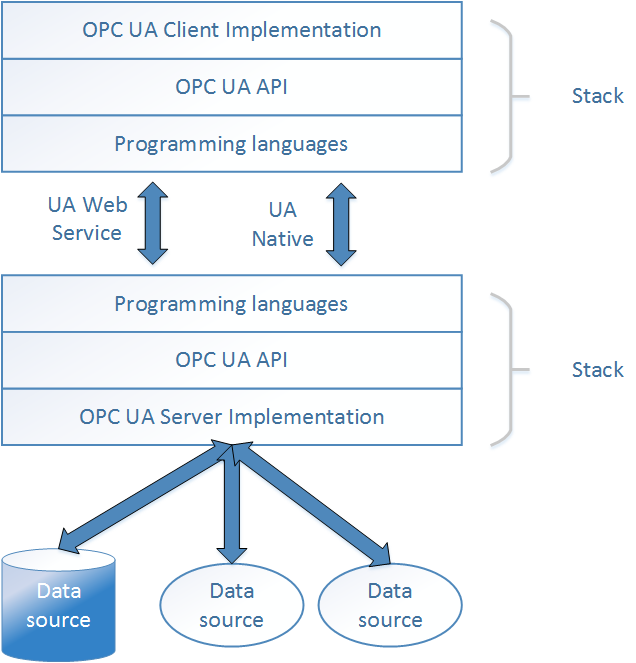
\includegraphics[width=.7\textwidth]{resources/images/OPCUA}
    \caption{The OPC UA Architecture inspired from~\cite{ua2}}\label{fig:contrib2:ua}
\end{figure}

In this context, an OPC UA client is implemented as an OPC UA communication stack. Since the OPC UA API used for accessing the communication stack can change from one operating system to another or from one programming language to another, it was not standardized. On the other hand, the client implementation should use it to access the stack~\cite{ua2}. Consequently, it is possible to develop a customized communication stack with a specific API.  \par

From the server's point of view, it is mainly responsible for delivering the request messages to the Server Implementation through an OPC UA API. This API might be the same as the API located in the OPC UA client. After receiving the request, the Server Implementation implements the logic required for returning an appropriate response message to the originator. Furthermore, as illustrated in the figure~\ref{fig:contrib2:ua}, it is possible for the OPC UA Sever Implementation to get the data from various underlying systems such as a configuration database or set of devices.\par 
Moreover, the OPC UA  aims to be more open for the different technologies used to develop an application, by defining services and concepts in an abstract manner. In this context, OPC UA specifies a technological mapping for implementation. The specified mappings address three main important tasks:
\begin{inlinelist}
  \item data encoding
  \item securing the communication and
  \item transporting the data.~\cite{bookua}
\end{inlinelist}
Currently, the OPC UA standard specifies two different mappings technologies: UA Web Services and UA Native~\cite{ua2}. While the first mapping technology uses SOAP, the second one uses only a simple binary network protocol. The OPC UA provides the possibility to encode the data. There are mainly two encoding approaches which can be adopted. Either by using XML or by using UA Binary. Each technique has advantages and disadvantages, but they are out of the scope of this thesis because the encoding of the data is independent of the mapping technologies.  \par 
Both of the approaches uses different protocols for mapping. The UA Web Service employs the SOAP/HTTP protocol while the UA Native mapping works on TCP/IP.  \par 
Furthermore, the OPC UA specification defines a concept for servers aggregation. Thus, an aggregating server is formed of one or more OPC UA server and publish the information on those servers. In this context, the client does not have to access each time multiple servers. Instead, it is able to access only one server that aggregates all the server needed.

\subsection{OMG Data Distribution Service}

The Data Distribution Service (DDS) is created by the Object Management Group (OMG) as a middleware protocol and API standard for the loT in order to enable interoperability among the connected things such as machines, mobile devices, and enterprise systems. This standard defines a data-centric connectivity by integrating the various components of a given system together in the aim of providing reliability, scalability and low latency data connectivity. It is possible to deploy the DDS standard on various platforms such as devices or the cloud. \par 
To ensure this flexible and modular structure, DDS decoupling location, time, message flow and platform from each other. This is mainly done by providing various methods. For decoupling the location, the DDS standard presents the anonymous publish/subscribe model. It also decouples the time from the other components by ensuring a time independent data distribution. Additionally, the DDS standard offers a data-centric connection management based on messages which allow the decoupling of the message flow among the different components of the system\cite{ssd2}. Finally, the DDS decouple the platform is done by supporting a platform independent model which is responsible for mapping the various models presented according to their platform. \par 
As illustrated in the figure~\ref{fig:contrib2:dds} the DDS standard define specific entities for communication and the relation between them. Those entities are described in the following:
\begin{figure}[htbp]
    \centering
    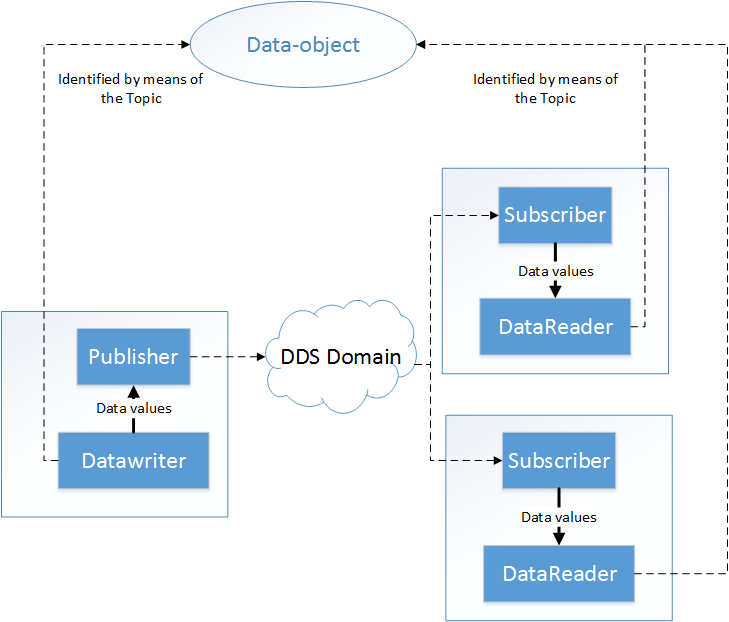
\includegraphics[width=.9\textwidth]{resources/images/dds}
    \caption{Overview of the Data Distribution Service standard inspired from~\cite{ssd} and~\cite{ssd3}}\label{fig:contrib2:dds}
\end{figure}
\begin{itemize}
\item \textbf{Domains:} the first entity is the domain which represents a virtual global data-space~\cite{ssd3} which provide information in a specific domain. Those information are accessible by all the application registered to the information domain.
\item \textbf{Publisher:} as defined in the DDS specification, the publisher is a well-defined object that is responsible for the distribution of different types of data.
\item \textbf{DataWriter:} for applications to communicate with a publisher they must use the DataWriter object. In this manner, when an application connects to a specific Publisher thought a DataWriter, the publisher should perform the distribution of data.
\item \textbf{Subscriber:} In contrast to the publisher, the subscriber is the entity responsible for receiving the published data. The subscriber is responsible as well for making the received data available for application. 
\item \textbf{DataReader:} it is required for the application to use the DataReader object in order to access the data received by the subscriber. From this perspective, subscription is defined by the a the association of a data-reader with a subscriber  which provide information about the intention of the application and which data it require in order to perform a subscription~\cite{ssd} 
\item \textbf{Topic:} This entity is used in order to make it easier for the subscriber to refer the required publication unambiguously. Thus, this object is defined to fit between publications and subscriptions.
\end{itemize}


\subsection{OneM2M Partnership Project}

OneM2M is a standard partnership project founded in 2012 by seven development organizations (SDOs) including TTA, ETSI, TIA,  ATIS,  TTC, ARIB, CCSA, and TDSI. Those participating organizations are working under the same objective which consists of transferring all standardization activities in the scope of IoT service layer to the oneM2M~\cite{onem2mC}. From this perspective, oneM2M standard partnership project aims at providing a single horizontal service platform for exchanging, sharing and manipulating data between various IoT applications which can be used in IoT industries by enabling smarter IoT services to users. Therefore, the oneM2M standard is creating various scalable and interoperable IoT standards to define the communication among things and services.\par 

OneM2M has been developing several specifications in the aim at enabling interoperability and inter-working. In contrast to the OMG Data Distribution Service and OPC UA standards, oneM2M is the only standard that developed a specification for enabling Semantic technologies to face the interoperability problem. In fact, Semantic technologies are specified by oneM2M to describe the meaning and information gathered from the oneM2M resources. Currently, oneM2M is developing standard documentations dedicated to interoperability and conformance testing~\cite{onem2ms}. \par 
In this section, the functional architecture of the oneM2M standard specification is provided as well as its key feature. Afterward, the approach used for inter-working is presented. Finally, the Semantic approach specified by oneM2M is discussed.



\subsubsection{OneM2M Functional Architecture}
In August 2014, oneM2M realised its first specification with a deployable IoT solution. Within this release, there are a set of common standards functions that enable the creation of a horizontal IoT service platform which are presented herein. The motivation behind the horizontal IoT platform is to allow various providers to work with a common framework~\cite{H} \par 

OneM2M standard specification compromise three different functions as depicts in the figure~\ref{fig:contrib1:goal}. The first function is the Application Entity (AE) which implements an M2M application service logic as specified in~\cite{onem2marchi}. Each instance executed by an application service logic is named Application Entity (AE) that can be resident in some M2M nodes and more than once on a single M2M node. The second function is Common Services Entity (CSE) which represents an instantiation of common service functions of the M2M environments. It offers several different service functions such as Data Management, Device Management, Subscription Management, and Location Services. The last function is the Network Services Entity (NSE) which provides services from different networks to the CSEs. In the context of the roles of Mca interface, it provides communication between different oneM2M CSEs~\cite{onem2marchi}.
\par
\begin{figure}[htbp]
    \centering
    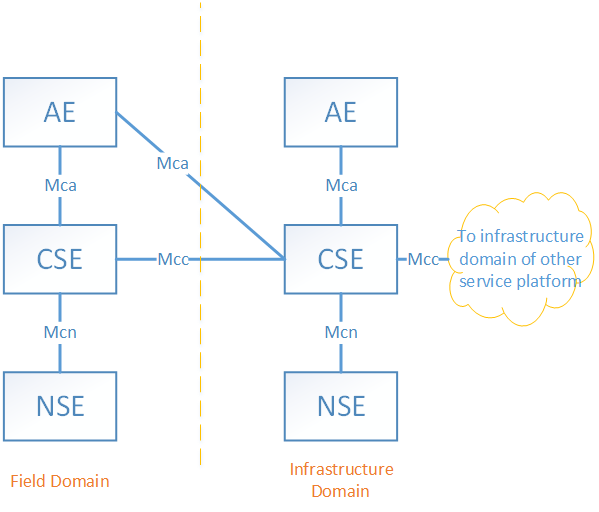
\includegraphics[width=.8\textwidth]{resources/images/arch}
    \caption{oneM2M Functional Architecture based on }\label{fig:contrib1:goal}
\end{figure}\par
There are a huge number of connected M2M and non-M2M enabled devices within an IoT network. Therefore the oneM2M standard specifies various functions to deal with this heterogeneous devices. Since that, in the modern word most of the devices connected to a given platform are more likely to face energy shortages, and they are often presented with limited storage capabilities, they can not interact immediately to all transaction with each other or with another component in the network, this situation will cause cancellation of the transaction and many other problems. Therefore, REST based architecture is considered within the the first release of oneM2M standardization. In fact, REST is based on the concept of resource addressed by URLs. Thus, it provides to the different devices connected to a given oneM2M system a way to store their states and data. In this manner, Applications that perform various transactions are able to use the internal subscription/notification mechanism specified by oneM2M to subscribe to a targeted resources and get notified by the CSE whenever the data is available or updated. An example of the oneM2M resource tree is illustrate in Figure~\ref{fig:contrib1:tree}. In this context, each device in the M2M system is presented by a uniquely addressable resource in the hierarchical tree. For example, a device can be presented by a <device\textunderscore name> resource under the hosting getaway resource <CSEBase>. Application in the other hand is presented by <Container> resource that includes one or more resource type container to classify different <contentInstences> resources under it, where the targeted data are generally located.\par
\begin{figure}[htbp]
    \centering
    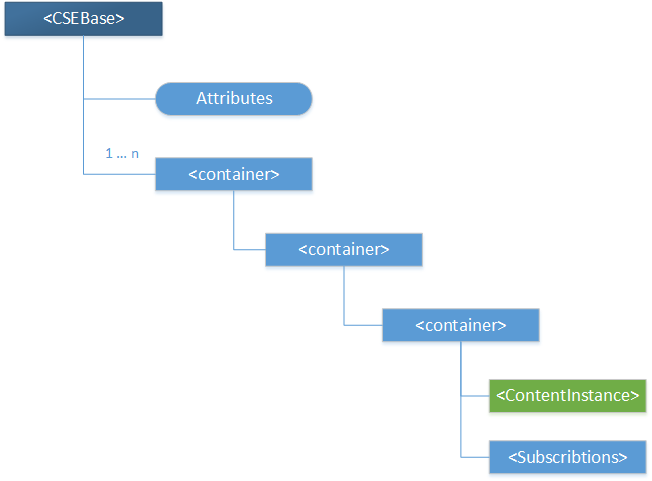
\includegraphics[width=.8\textwidth]{resources/images/tree}
    \caption{M2M Resource Tree based on oneM2M specifications}\label{fig:contrib1:tree}
\end{figure}
Moreover, the oneM2M standard specify as well a publish/subscribe architecture, which facilitate the exchange between sensor networks and cloud-based networks. The publish/subscribe architecture presents a dynamic network pattern to deliver sensor driven processed data to subscriber. It also create a decoupling communication between publisher and subscriber based on time, space and control flow. (Add Request Routing)\par
An interworking proxy entity is introduced to interconnect various local connectivity protocols

\subsubsection{Interworking Proxy Entity}
In order to provide means for interworking with non-oneM2M enabeled devices which generate a huge amount of data, the oneM2M standardization introduce an interworking proxy entity (IPE) to interconnect different local connectivity protocols such as ZigBee or ICE. As illustrated in the figure~\ref{fig:contrib1:goal}, the interworking proxy entity is defined by oneM2M as a specialized AE for interworking with non-oneM2M system as showing in the figure. IPE includes two main functionalities:  
\begin{itemize}
\item translate a non-M2M interface non-oneM2M protocols and massages to oneM2M ones via the Mca interface
\item Mapping non-oneM2M data models into oneM2M resources, which are eventually exposed to oneM2M services.
\end{itemize}\par
In this context, for each new local connectivity protocol a dedicated IPE should be created. 
\begin{figure}[htbp]
    \centering
    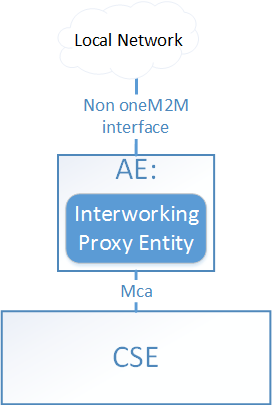
\includegraphics[width=.4\textwidth]{resources/images/ipe}
    \caption{The Interworking Proxy Entity}\label{fig:contrib1:goal}
\end{figure}
\subsubsection{Semantic Interoperabiltiy Enablement in OneM2M}
The oneM2M architecture provides procedures to discover the different resources available in a specific CSE within a given M2M system. This procedure is knowing as the resource discovery procedure (TS-0018). It is mainly processed using the RETRIEVE method which retrieves the information presented or stored in the resource's attributes. This can be done by sending a request from a specific originator (e.g. CSE or AE) to a given receiver by including the name of the target attribute in the Content parameter in the request message. When receiving the request, the receiver verifies the presence of the requested resource and checks the originator privileges for retrieving the information related to the resource. The Receiver returns the requested information only if the verification is successfully done. Otherwise, an error is returned instead. Figure TS-0018 present the mentioned procedure for retrieving a given resource.\par
Moreover, as specified in oneM2M-TS-0001 oneM2M Functional Architecture version 3, the usage of the resource discovery procedures can be customized with specified Filter Criteria parameter which limits the scope of the results. To be more specific, the filter criteria parameter provides rules description for resource discovery, (e.g. creation time, resource types, etc.).\par
Using the conventional oneM2M service layer mechanisms together with the filter criteria can provide effective resource discovery, however, it is not as advanced as expected for querying resources. Therefore, the second release of the oneM2M standard specification aims at realizing semantic-based query by annotating the target resources semantically. OneM2M enable the semantic technologies within a given oneM2M system by adding as a child resource the semantic representation of the parent resource. In this manner, all the resources provide a specific semantic representation which allows more advanced query based on semantic.\par
As defined in the oneM2M specification documentation TR-0007-Study on Abstraction and Semantics Enablement version 2.9, the type of the resources aiming at providing a semantic representation of target resources, is <semanticDescriptor> which will be discussed in more details herein. This type of resources allows the storage of the semantic description which includes relationship and information of a given resource in its child resource. Storing the different semantic information in the <semanticDescriptor> resources allows the extraction and the storage of this information in a semantic repository. The semantic repository contains mainly a set of triples allowing semantic-based query execution. The main architecture of the semantic annotator instance or the resource type <semanticDescriptor> consist of associating this type of resources with the resources that is included in it's tripled. \par
\begin{figure}[htbp]
    \centering
    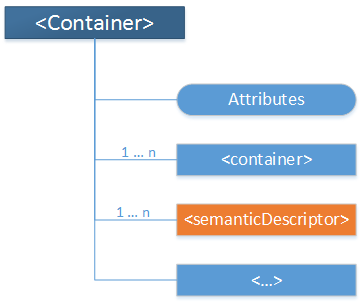
\includegraphics[width=.5\textwidth]{resources/images/sdresource}
    \caption{oneM2M Resource Tree including resource type < semanticDescriptor> }\label{fig:contrib1:goal}
\end{figure}

\sidenote{Integration}
According to the oneM2M specification, each resource in the M2M system includes one or more attribute. This attributes comprises information pertaining to the resource. Moreover, each attribute has a unique name that belongs only to a given resource and value. The resources attribute are uniquely addressable as well.\par  %In the table, a set of common attributes of M2M resources is presented. 
In the oneM2M standard specification, those attributes are commonly used by all announced resources including the resource type semantic descriptor. Besides the common attributes, there are more specific attributes for the semantic descriptor. Those attributes are shared by all announced < semanticDescriptor > specializations.\par
As specified in oneM2M TS-0004 Service Layer Core Protocol Version 2.7.1, semantic descriptor resource includes five mandatory and optional attributes as showing in the figure.
\begin{figure}[htbp]
    \centering
    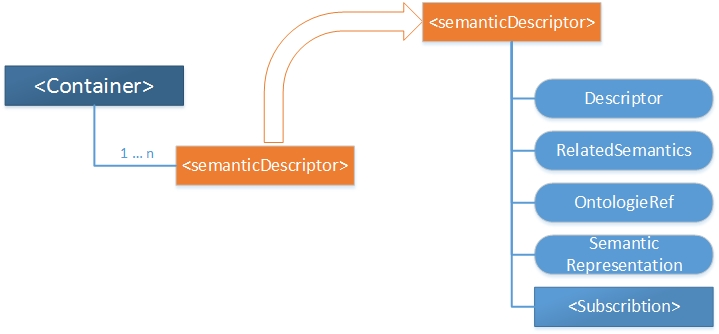
\includegraphics[width=1\textwidth]{resources/images/sdattribute}
    \caption{Structure of <semanticDescriptor> resource }\label{fig:contrib1:goal}
\end{figure}
\subsubsection{Mandatory attributes}
Mandatory attributes mean that in case one of this attributes is missing while creating the resource type semantic descriptor, an error would be throwing back, and the creation of the resource is abandoned.
Those attributes are: 

\paragraph*{Descriptor attribute:}

Each semantic descriptor must provide exactly one descriptor attribute. This attribute is responsible for storing the semantic description of the resource whose child resource the <semanticDescriptor> resource is. As mentioned previously, a semantic description is mainly provided by different ontologies within the semantic annotator architecture. More specifically this description shall be according to subject-predicate-object triples as defined in the RDF graph-based data model [4]. The encoding of the RDF triples used in oneM2M is xs:base64Binary as defined in oneM2M TS-0004 Service Layer Core Protocol Version 2.7.1[TS-0004]. Base64Binary is a representation of arbitrary Base64 encoded binary data. To be more specific data in the base64Binary format are encoded using Base64 encoding defined in RFC 4648 [9], which is derived from in RFC 2045 [10].
\paragraph*{RelatedSemantics attribute:}

For creating a new semantic descriptor resource about a resource and potentially subresource within the semantic annotator design, the semantic descriptor resource must contain exactly one related Semantic attribute. As indicated in its name this attribute provide a list of URIs for resources containing related semantic information to the resources where it was created. The URI(s) aims at referencing other <semanticDescriptor> resources. This attribute is importance because it provides means to execute SPARQL queries. This attribute will be presented and explained in more detail in the data access section.
\paragraph*{DescriptorRepresentation attribute:}
Each semantic descriptor must provide exactly one DescriptorRepresentation attribute. This attribute specifies the serialization type of the descriptor attribute. It has a fixed value application/rdf+xml:1 which consist of a string composed of a media type followed by an m2m:encoding separated by ":" character. 
\subsubsection{Optional attributes}
As defined in oneM2M TS-0004 Service Layer Core Protocol Version 2.7.1[TS-0004], resource of type <semanticDescriptor> can have one or more optional attribute that provide further information depending on the M2M system.
\paragraph*{SemanticOpExec attribute:}
The semanticOpExec attribute contains a SPARQL update request which aims at updating the descriptor attribute. Thus, it is not created or retrieved. 
\paragraph*{OntologyRef attribute:}
 The ontologyRef attribute provide a reference URL of the ontology used to semantically describe the information that is stored in the descriptor attribute. Hence, it is highly recommended to use this attribute in case the information can be described using more than one ontology.\par
The table below summarize all the specific attributes of the semantic descriptor resource.

\begin{sidewaystable}
\centering
\caption{Attributes of the semantic descriptor resource}
\label{my-label}
\begin{tabular}{llllll}
\hline
\textbf{<SemanticDescriptor> attributes}                              & \textbf{Role}                                                                                                                                                                      & \textbf{Data type}                                                                  & \textbf{Default value}                                                    & \textbf{Mandatory}             & \textbf{Optional}              \\ \hline
\textbf{descriptorRepresentation} & \begin{tabular}[c]{@{}l@{}}specify the serialization \\ type of the descriptor\\ attribute\end{tabular}                                                                   & \begin{tabular}[c]{@{}l@{}}Semantic content \\ representation\end{tabular} & \begin{tabular}[c]{@{}l@{}}application/\\ rdf+xml:1\end{tabular} & \multicolumn{1}{c}{X} &                       \\\midrule
\textbf{semanticOpExec}           & \begin{tabular}[c]{@{}l@{}}Update the descriptor \\ attribute\end{tabular}                                                                                                & SAPRQL                                                                     &                                                                  &                       & \multicolumn{1}{c}{X} \\\midrule
\textbf{descriptor}               & \begin{tabular}[c]{@{}l@{}}Storing the semantic \\ description of the targeted\\ resource\end{tabular}                                                                    & \begin{tabular}[c]{@{}l@{}}base64Binary \\ encoded data\end{tabular}       &                                                                  & \multicolumn{1}{c}{X} &                       \\\midrule
\textbf{ontologyRef}              & \begin{tabular}[c]{@{}l@{}}Provide a reference URL \\ of the ontology used to\\ semantically \\ describe the information \\ in the descriptor attribute\end{tabular}      & URL                                                                        &                                                                  &                       & \multicolumn{1}{c}{X} \\\midrule
\textbf{relatedSemantics}         & \begin{tabular}[c]{@{}l@{}}Provide a list of URIs \\ for resources containing\\ related semantic \\ information to the\\  resources where \\ it was created.\end{tabular} & List of URL                                                                &                                                                  & &   \multicolumn{1}{c}{X}                      \\\hline
\end{tabular}
\end{sidewaystable}

\section{Semantic in the Internet of Things}\index{Related Area 3}
Based on the introduction of this thesis, it is necessary to provide the semantic information of things in order to reach the ultimate goal of the Internet of Things. This need for semantic technologies in IoT in order to discover data and resources was identified by the Strategic Research Agenda (SRA) in 2010~\cite{booksd}. During the past years, semantic web technologies gained a big attention in many fields. Besides providing an efficient solution to the interoperability problem among things in IoT, semantic web technologies has proven their capabilities to link related data as well~\cite{booksd}.\par 
Thus, using semantic web technologies at the early staged of the IoT, provide means for the future research to build the concept of Linked Open Data on the earlier integration of ontologies (e.g., lightweight ontologies) into IoT infrastructures and applications. From this perspective, within this section, an introduction to the Semantic web technologies is presented as well as the explanation of the term ontology and its uses.

%SEMANTIC IN IOT The 2010 SRA has identified the importance of semantic technologies towards discovering devices, as well as towards achieving semantic interoperability. During the past years, semantic web technologies have also proven their ability to link related data (web-of-data concept) [48], while relevant tools and techniques have just emerged [49]. Future research on IoT is likely to embrace the concept of Linked Open Data. This could build on the earlier integration of ontologies (e.g., sensor ontologies) into IoT infrastructures and applications. Semantic technologies will also have a key role in enabling sharing and re-use of virtual objects  as a service through the cloud, as illustrated in the previous paragraph. The semantic enrichment of virtual object descriptions will realise for IoT what semantic annotation of web pages has enabled in the Semantic Web. Associated semantic-based reasoning will assist IoT users to more independently find the relevant proven virtual objects to improve the performance or the effectiveness of the IoT applications they intend to use.
%2.11.4.1 IoT interoperability necessary framework
%2.5.3. http://www.internet-of-things-research.eu/pdf/Converging_Technologies_for_Smart_Environments_and_Integrated_Ecosystems_IERC_Book_Open_Access_2013.pdf

\subsection{Semantic Web technologies }
The director of the World Wide Web Consortium (W3C) and the inventor of the World Wide Web Tim Berners-Lee together with James Hendler and Ora Lassila published the first article that features the "Semantic Web" in May 2001~\cite{hi}~\cite{rb}. This article presents a novel way to use and search the Internet which can be seen as a new dimension that provides new opportunities and possibilities. Since HTML provides means to store visual information, it is rather designed for human and computers. Thus, it is not possible for computer or search engine to read and understand the text of an HTML web page. \par 
From this perspective, the Semantic Web aims at extending the current World Wide Web to focus on technology as well as human. Thus, in contrast to the World Wide Web, the Semantic Web does not require a human presence. It uses the natural languages to search compile and organize information from the Web. Therefore, the human presence in the Semantic Web is only required to initiate a request. This approach would enable, for example, machine agents to intelligently search the Web, create decisions and accomplish tasks on behalf of humans~\cite{rb}.
As illustrated in the figure~\ref{fig:contrib2:stack} the architecture of semantic web consists of various layers where each layer uses the capabilities of the layer below. 
\begin{figure}[htbp]
    \centering
    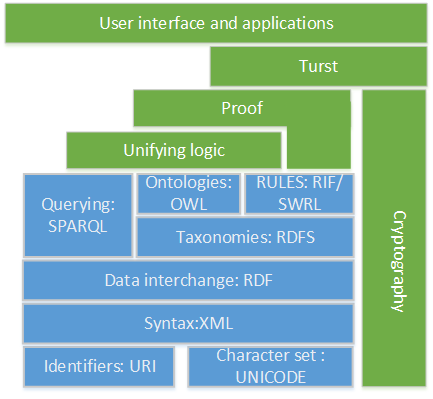
\includegraphics[width=.6\textwidth]{resources/images/stack}
    \caption{Semantic Web Stack based on~\cite{layer}}\label{fig:contrib2:stack}
\end{figure}
The bottom layers of the stack which are highlighted in blue indicate the components of the semantic web that have been standardized. In the other hand, the upper layers highlighted in light green are not clear yet how to implement them, but they are still required for a sufficient deployment of Semantic Web~\cite{layer}. \par
The first layer which consists of the URI and Unicode follows the important features of the existing Web. In fact, international character sets are encoded using the Unicode standard which allows the usage of human languages on the web. The URI refers to Uniform Resource Identifier which consists of a string of a standardized form that provides means to uniquely identify resources. The URL includes two subsets: the Uniform Resource Locator (URL) and Uniform Resource Name (URN). It is important to use URI(s) to guarantee the distribution of the Internet system~\cite{layer2}. \par 

Extensible Markup Language (XML) layer ensure a common syntax usage in the Semantic Web~\cite{layer2}. Thus, the use of XML allows the description of data in a way that is both human and machine-readable. Furthermore, XML includes various applications such as the Resource Description Framework (RDF) which is the core data representation format for Semantic Web. \par

As it was mentioned previously, RDF is the core data representation format for Semantic Web~\cite{thesis}. It is a framework that allows the description of the information in a graph form. XML and Turtle (TTL) can both be employed as the normative syntax for serializing RDF. The base of RDF is the usage of triples (subject, predicate, and object) that form a graph of data. Thus, all information in the Semantic Web is described through the RDF language. Each subject and predicate are denoted by a unique Uniform Resource Identifier (URI), generally a Uniform Resource Locator (URL). In the other hand, the object can either be a literal or a URI. From this perspective, it is possible to form a directed graph, as shown in Figure~\ref{fig:contrib2:rdf}, where objects are represented using literal and URI. Furthermore, it is possible to use RDF/XML to serialize the graph. In fact, various formats can be used for serialization such as JSON/JSON-LD, N3, and N-Triplets. There are common concepts presented by the RDF specification such as blank nodes and collections.
\begin{figure}[htbp]
    \centering
    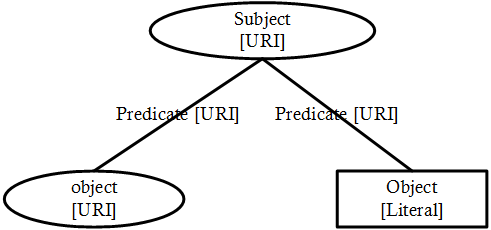
\includegraphics[width=.5\textwidth]{resources/images/rdf}
    \caption{Types of RDF triples}\label{fig:contrib2:rdf}
\end{figure}
Since that RDF provides possibilities to represents graphs formed by triples, it is possible to almost anyone to define the vocabulary of terms used for more detailed description. In this context, RDF Schema (RDFS) is created to provide a standardization for taxonomies and ontological constructs description. Thus, RDFS enable the creation of lightweight ontologies through describing taxonomies of classes and properties~\cite{rdfs}. In fact, all resources are divided into groups called classes. In the same way, classes are also resources. Therefore they are identified by URIs, and they are described using properties. Each member of a class is called instance, which is stated using the rdf:type property. Moreover, RDFS define all resources as an instance of the class rdfs:Resource, all classes as an instance of rdfs:Class and subclasses of rdfs:Resource. Concerning the properties they are defined as instances of rdf:Property which presents relations between subjects and objects in RDF triples such as rdfs:subClassOf or rdfs:label. \par
In order to create more complex ontologies, it is required to use the Web Ontology Language (OWL) which is derived from description logics. The OWL offers more constructs over RDFS by providing additional standardized vocabulary~\cite{owl}. As showing in Figure~\ref{fig:contrib2:owl}, there are three species of OWL:
\begin{inlinelist}
  \item OWL Lite for taxonomies and simple constrains
  \item OWL DL for full description logic support
  \item and OWL Full for maximum expressiveness and syntactic freedom of RDF.~\cite{owl}
\end{inlinelist}\par 
\begin{figure}[htbp]
    \centering
    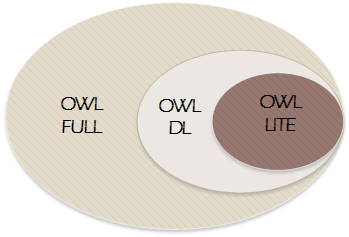
\includegraphics[width=.5\textwidth]{resources/images/owl}
    \caption{the relationships between OWL species based on~\cite{owlpic}}\label{fig:contrib2:owl}
\end{figure}
OWL Lite is the simplest OWL language used to express taxonomy and simple constraints. On the other hand, OWL Full is the most complex OWL language formed by the full OWL vocabulary~\cite{owl}. Thus it has no expressiveness constraints which allow complex expressions. OWL DL provide means to use the knowledge representation formalism Description Logics (DL) which are a family of formal knowledge representation languages used for defining general ontologies~\cite{dl}. Hence, OWL DL in one hand support maximum expressiveness, and in the other, it retains computational completeness by providing description logic capabilities. As showing in the figure~\ref{fig:contrib2:owl}, each legal OWL Lite ontology can be considered as a legal OWL DL ontology, in the same manner, each legal OWL DL ontology is seen as a legal OWL Full ontology. Generally, the inverse of this relation do not hold~\cite{owlpic}.\par 

For performing queries on RDF data, RDFS and OWL ontologies with knowledge bases, the SPARQL Protocol And RDF Query Language (SPARQL) are available[]. SPARQL is an SQL-like language used to query ontologies such as RDFS and OWL. It used RDF triples for the matching part as well as the returned results. Thus, the TURTLE syntax is used in order to express RDF graphs in the matching part of the SPARQL query~\cite{thesis}. SPARQL is considered a protocol for accessing RDF data as well.\par 
 
Based on the figure~\ref{fig:contrib2:stack}, it is expected that all the semantics and rules are performed within the layers underneath Proof. Thus, the results are used to prove deductions. The trust layer means that the proof and the trusted inputs signify that the results are trustful. Finally, cryptography is used in order to provide reliable inputs.

\subsection{The Semantic Web Technologies stack for IoT}
Figure~\ref{fig:contrib2:stack2} debate an overview on how Semantics can be used at various levels in IoT. The figure was adapted from ~\cite{stacksemantic2}in order to illustrate the Stack presented by the Semantic Web Technologies for IoT. \par 
Based on the figure, there are three main levels where the Semantic Web technologies can be integrated~\cite{stacksemantic1}. The first level is the "modeling level" which aims at providing a common understanding the capacities, characteristics, and relations of Things. Thus, integrating Semantic Web
technologies at this level enable the use of shared and accepted vocabularies and lightweight ontologies which facilitate the integration of data generated by a various system. Such an integration of vocabularies and ontologies in the "modeling level" can be done by using a sensor ontology to describe the sensor data collected. The second level is the "data processing level." Using Semantic Web technologies within this level enable reasoning and inference over the data~\cite{stacksemantic1}. To be more specific, this level requires the use of description logic and OWL semantics described in the previous section. The third level is the IoT Services and Application". Enhancing this level with the Semantic Web technologies by using specific ontologies and description enable the discovery, publication, and composition of services in IoT.
\begin{figure}[htbp]
    \centering
    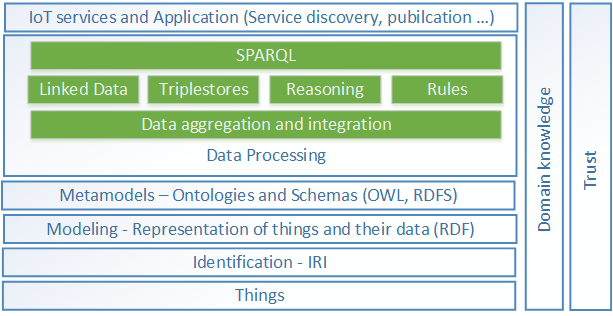
\includegraphics[width=1\textwidth]{resources/images/stacksemantic}
    \caption{The Semantic Web Technologies stack for IoT adapted from~\cite{owlpic}}\label{fig:contrib2:stack2}
\end{figure}

\section{Ontologies for the Internet of Things}

As presented in the previous section, ontologies provide a distributed and common description of various domains communicated between people and application systems. Since ontology aims at providing a consensual domain knowledge, its development involve a various cooperation between different people possibly located at different locations.\par 
In this context, there are already different projects working on ontologies and vocabularies indexation on the Web. Currently, the most popular schemas on the Web is Schema.org which is a collaborative and community work aiming at creating, supporting and promoting schemas for structured data on the Web~\cite{stacksemantic1}. At the time of writing, schema.org is used by more than 10 million sites in order to markup their pages and email messages~\cite{schema}. Although schema.org provide full descriptions for general and commonly used aspect such as Places, relationships, Person, etc., it does not provide specific IoT domain concepts such as Sensor concept.\par 

Thus, currently, many research and works aim at providing a vocabulary specified for IoT. At the time of writing, there are already 300 IoT-specific vocabularies presented in the Linked Open Vocabularies (LOV) online catalog maintained at~\cite{site}. The Open Knowledge Foundation creates the Linked Open Vocabularies in order to facilitate the research process of the various type of vocabularies dedicated for data description on the Web~\cite{rfr}. Evaluating and comparing 300 ontologies is out of the scope of this thesis and will be reserved for future work. However, the most relevant and well-referenced ontologies in other works are presented herein. \par 

One of the most well-knowing ontologies in the field of IoT is the Semantic Sensor Network Ontology (SSN) developed and maintained by the W3C Semantic Sensor Network Incubator Group in 2011~\cite{ssn}. The full ontology inherits its 41 concepts and 39 object properties directly from 11 DOLCE Ultra Lite (DUL) concepts and 11 DUL object properties~\cite{ssn}. SSN ontology is able to describe sensors, their capabilities, observations and methods for sensing~\cite{ssn}. Moreover, the SSN ontology includes various concepts for operating and a structure for field deployments which describes the deployment lifetime. This ontology is built on a central Ontology Design Pattern (ODP). This design aims mainly at describing the relationships between sensors, stimulus, and observations referred to as the Stimulus-Sensor-Observation pattern.
The SSN ontology can be presented using four different perspectives~\cite{ssn}: 
\begin{itemize}
\item \textbf{Sensor perspective:} this perspective focus on the output of the sensors, what is this output and how it was sensed. 
\item \textbf{Observation perspective:} this perspective concentrate only on the observed data and related metadata.
\item \textbf{Property perspective:} which focus on the observations that have been made about a particular property.
\end{itemize}
This ontology takes on consideration an inclusive view of what a sensor is. A sensor is defined in the SSN ontology as anything that observes. Furthermore, SSN allows for each sensor to have a hierarchical representation using ssn:hasSubSystem object property~\cite{rfr}. This representation is illustrated in the Listing~\ref{lst:contrib3:rw1}. Although SSN is considered a “5 star” ontology which follows all the rating requirements, it does not provide means to represent the concept of Actuators~\cite{rfr}. It also does not include various material such as units, locations, and hierarchies of sensor types~\cite{ssn}. \par 

\lstset{caption=An example of a System with a Temperature Sensor and a Pressure Sensor, label=lst:contrib3:rw1,
language=xml, breaklines=true, numbers=left, basicstyle=\small\ttfamily,
stepnumber=1, frame=single, inputencoding=utf8/latin1}~\lstinputlisting{resources/code/ssn.rdf}

Besides the SSN ontology, there are various specialized information models defined for the IoT such as the Zigbee or KNX data models. The SSN ontology, as well as those specialized ontologies, suffer from two main issues. Either those ontologies are too specialized to be used in different scenarios because they concentrate on a particular application domain or they lack some important concepts such as the lack of actuator representation within the SSN ontology. For those reasons, multiple ontologies are constructed from those ontologies in order to handle the missing concepts or to be more generalize to allow the usage of the ontology by different stakeholders. Thus, in this thesis, there are two main ontologies considered which are not very specialized and offer all the essential concepts for the data annotation. The first ontology considered is the Fiesta-IoT Ontology which is an EU project that comprises 14 partners and integrates previous and ongoing EU projects already using semantic web technologies~\cite{fiesta1}. Fiesta-IoT Ontology is a collection of merged concepts from different exciting ontologies such as the SSN ontology previously presented, IoT-lite, M3-lite Taxonomy, Time and DUL. The second ontology considered is the oneM2M Base ontology specified by the oneM2M standard specification in TS012~\cite{baseontology}. Since the design discussed within this thesis rely mainly on the oneM2M specification, it is more beneficial to use the ontology specified by the standard.


\section{OpenMTC Platform}

OpenMTC platform~\cite{openmtc} is an M2M solution for the Internet of Things created and developed by The Fraunhofer FOKUS and Technical University of Berlin (TUB). This platform is considered as an implementation of the oneM2M standard specification which has been designed as a horizontal layer spanning across multiple vertical domains (e.g., Smart transport, eHealth, etc.). The OpenMTC platform support integration of heterogeneous sensors which allows the applications developers to use and manipulate various heterogeneous devices and sensors. Thus, with its concept, OpenMTC platform enable academia and industry to deploy it independently or as part of a common platform.\par 

Currently, this platform is moving toward an intelligent fog node framework called OpenIoTFog~\cite{openiotfog} where the semantic interoperability is required. Therefore, this work aims at moving the OpenMTC towards the OpenIoTFog by providing semantic interoperability which can be done thanks to the oneM2M standard specification implementation within the platform. \par 
As discussed previously, the oneM2M standard specification is one of the fewer standardization efforts that follows the semantic interoperability approach by specifying methods and concepts in this regards. Hence, the OpenMTC platform is considered within this thesis as the perfect candidate for implementing semantic technologies for two main reasons. First, as mentioned in the previous paragraph, the OpenMTC platform provide various possibilities to interact and collect data from many heterogeneous oneM2M and non-oneM2M enabled sensors and devices. Thus, the interoperability problem is a real threat to the platform that should be handled. Second, the OpenMTC platform provides a full implementation of the oneM2M standard specification. Therefore it is possible to apply the semantic technologies on the platform by using the second release of the oneM2M specifications which provide a full description of the semantic implementations within a oneM2M platform. \par
This section presents an understanding of the OpenMTC platform architecture and its mains features.

\subsection{System Architecture}
The architecture of the OpenMTC platform adapts the high-level functional architecture specified by oneM2M which mainly consist of two service capability layers. A gateway service capability layer (GSCL) and a network service capability layer (NSCL). Those layers have been defined and specified by the ETSI Technical Committee M2M. The architectural design of OpenMTC run the different modules on an event based platform following the event based library concept Gevent which provide asynchronous I/O API that can scale its number of execution units according to the processing load. In Figure~\ref{fig:contrib2:openmtc}, the architecture of the OpenMTC is illustrated. As showing in the figure, OpenMTC mainly consists of a back-end M2M capability layer and a front-end M2M capability layer which follows the oneM2M standards as well as the ETSI Technical Committee. The front-end and back-end nodes are capable of using several transport protocols, such as HTTP, CoAP, and Websockets. As illustrated in Figure~\ref{fig:contrib2:openmtc}, it is possible to control the communication and interaction between the front-end and the back-end of the OpenMTC platform using the connectivity management layer over managed and unmanaged Access Networks. Thus, this layer is mainly responsible fort the communication establishment and messages forwarding. Furthermore, the core architecture of the OpenMTC platform includes the principle functionality defined by the oneM2M CSEs along with a set of application enablement APIs that allows the development of applications by third party.\par
\begin{figure}[htbp]
    \centering
    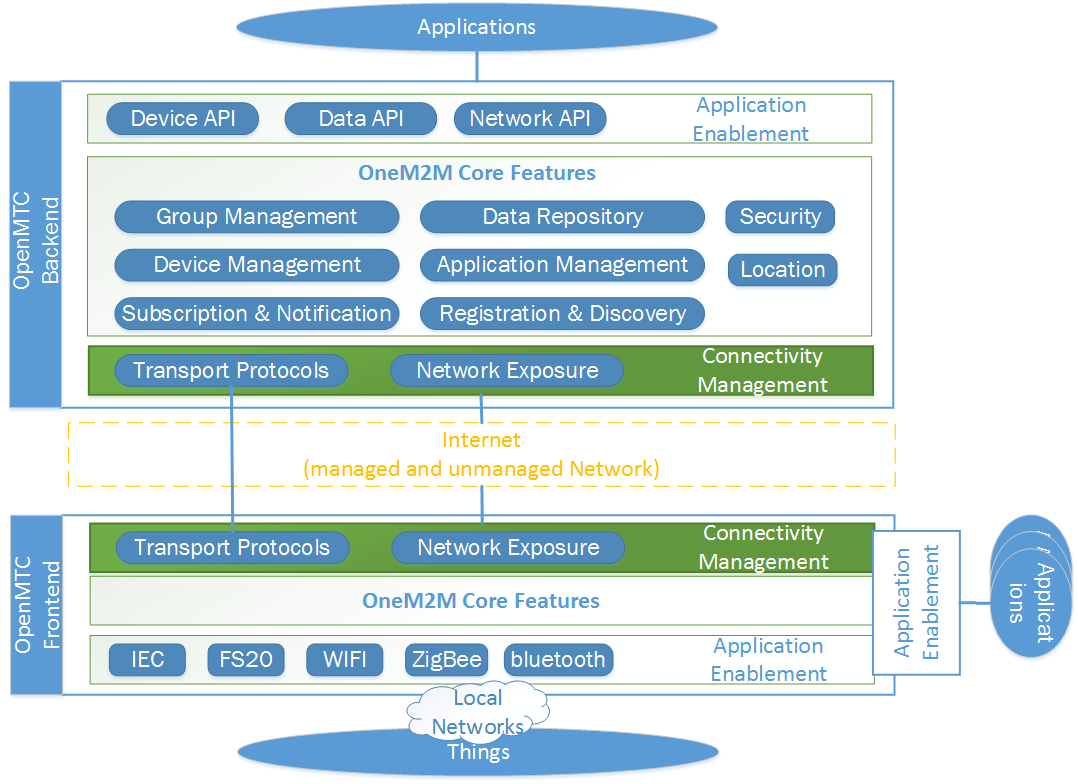
\includegraphics[width=1.1\textwidth]{resources/images/openmtc}
    \caption{The OpenMTC Platform Architecture based on~\cite{owlpic}}\label{fig:contrib2:openmtc}
\end{figure}
Furthermore, the client/server based RESTful architecture with the hierarchical resource tree defined by oneM2M are supported within the core architecture of the OpenMTC platform. Thus, using those features, it is possible for each device, sensor or "thing" to connect and store its states and data in the platform. Another characteristic of the OpenMTC platform is the separation of the communication over the platform interface and the transport protocol. Following the oneM2M standard specification, the OpenMTC platform offers a subscription and notification mechanism through its Addressing and Repository (RAR) capability which facilitate the management of the things connected to the platform~\cite{openmtc}. Using this mechanism provide various applications and services as well as the OpenMTC platform with the possibility to subscribe to a targeted resources and each time the resource subscribed to is modified they get notified.\par 
 In order to provide possibilities to interact with various heterogeneous sensors, devices or things, the OpenMTC platform provides different inter-working proxies entities that follow the oneM2M standard specification. Each IPE is responsible for one specific technology such as ZigBee or IEC which control the external devices by mapping them into the M2M resource tree structure. Thus, it is possible within the core design of the platform to integrate a specific IPE as needed.

\subsection{OpenMTC Key Features}
Based on the previous subsection it is possible to identify the key feature of the OpenMTC platform. Those features are highlighted in the following:
\begin{itemize} 
\item \textbf{OpenMTC Back-end:} There are various features provided by the back-end of the platform.  It offers a real-time data aggregation and processing as well as a well-defined device management and discovery system. As explained previously the core design of the back-end support as well different deployment scenarios. Finally and most importantly, it is possible within the openMTC back-end to develop IoT and M2M applications over a common platform. 
\item \textbf{OpenMTC Front-end:} This M2M capability layer provide various key feature as well. First and most importantly, it offers various possibility to support various sensors and actuators such as FS20, ZigBee or Bluetooth. This layer support also the use of different gateways such as Android-based gateways or Linux-based gateways.
\item \textbf{M2M Communication:} As it was mentioned previously, there are different ways of communication within the OpenMTC platform. The platform support open REST APIs and various communication protocols such as HTTP, MQTT or CoAP. The wireless access within the openMTC is supported as well.
\item \textbf{Scalable and Flexible:} The scalability of the platform is supported by its cloud-enabled deployment which is defined in one complete M2M solution. Moreover, the platform offers more flexibility through the separation of the functional elements available.
\end{itemize} 
\section{Conclusion}

\sidenote{Summary}
\todomid{write}

\sidenote{Takeaway 1}
\todomid{write}

\sidenote{Takeaway 2}
\todomid{write}

\sidenote{Takeaway 3}
\todomid{write}

\sidenote{Next chapter}
\todomid{write}
The idea behind this approach is to both optimize the query execution process and also to provide a way to perform a semantic query on the discovered semantic descriptors presented in the hierarchical resource tree without requiring the creation of a local temporary semantic graph store to put all the semantic triples extracted from the targeted resources.